\documentclass[10pt,a4paper]{article}
\usepackage[textwidth=450pt]{geometry}
\usepackage[utf8]{inputenc}
\usepackage{amsmath}
\usepackage{amsfonts}
\usepackage{amssymb}
\usepackage{hyperref}
\usepackage{graphicx}
\graphicspath{ {./images/} }

\author{Andrei Cristian\\\url{mailto:andrei.cristian1@info.uaic.ro}}
\title{Lab 3 - Exercise 4}

\begin{document}
%%%%%%%%%%commands%%%%%%%%%%
\newcommand{\llbracket}{[\![}
\newcommand{\rrbracket}{]\!]}
%%%%%%%%%%commands%%%%%%%%%%
\maketitle
\section{Exercise 6}
For the Labelled Transition System below, compute the following sets of states:

\begin{figure}[ht]
\centering
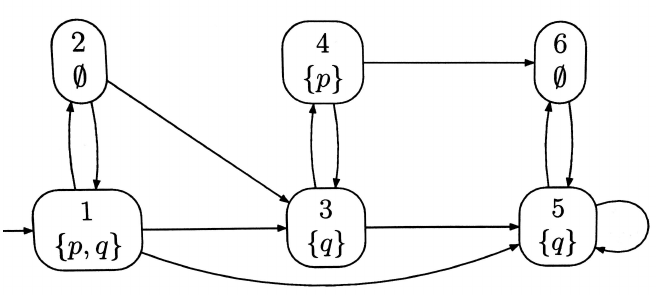
\includegraphics[scale=0.6]{ex4_labelled_transition_system.png}
\end{figure}

\begin{enumerate}
\item $\llbracket EFp \rrbracket$
\item $\llbracket AFq \rrbracket$
\item $\llbracket \varphi \rrbracket$, where $\varphi = E( q{U} (p \wedge \neg q )$
\item $\llbracket \varphi \rrbracket$, where $\varphi = EGq \vee ( EGp \wedge EFq )$
\end{enumerate}

\section{Solving of exercise 6}
Elementary temporal modalities that are present in the most temporal logics inlude the operators:\\
\textbf{$F(\lozenge)$ "eventually"} (eventually in the future)\\
\textbf{$G(\square)$ "always"} (now and forever in the future)\\\\
\textbf{{\large Definition(Semantics of CTL and CTL*)}}\\
Let $\pi=s_0,s_1,...$ be a path and $\varphi$ a $CTL*$ formula. If $\pi_i$ is the suffix of $\pi$ starting from position $i$,
\begin{itemize}
\item $\pi, i \models \top$
\item $\pi, i \models p$ iff $p \in L(s_i)$
\item $\pi, i \models \neg \varphi$ iff $\pi, i \not \models \varphi$
\item $\pi, i \models \varphi_1 \vee \varphi_2$ iff $\pi, i \models \varphi_1$ or $\pi, i \models \varphi_2$
\item $\pi, i \models X\varphi$ iff $\pi, i+1 \models \varphi$
\item $\pi, i \models \varphi_1 \mathcal{U} \varphi_2$ iff $\exists j \geq 0$ such that $\pi, j \models \varphi_2$ and $\pi, k \models \varphi_1$ for all $0 \leq k < j$
\item $\pi, i \models E\varphi$ iff there is an infinite path $\pi'=s_0',s_1',s_2',...$ s.t. $s_0'=s_i$ and $\pi', 0 \models \varphi$
\item $\pi, i \models A\varphi$ iff for every infinite path $\pi'=s_0', s_1', s_2',...$ s.t. $s_0'=s_i$, we have $\pi', 0 \models \varphi$
\end{itemize}
\textbf{{\large Solving Model Checking Problem}}\\
Let define:
\[ pre_\exists(Y) = \{ s \in S \mid \exists s' \in Y \textsl{ s.t. } (s, s') \in \mathcal{R} \} \]
\[ pre_\forall(Y) = \{ s \in S \mid \mathcal{R}(s) \subseteq Y \} \]
Compute $\llbracket \varphi \rrbracket = \{s \in S \mid s \models \varphi \}$
\[ \llbracket p \rrbracket = \{ s \in S \mid p \in L(s) \} \]
\[ \llbracket \neg \varphi \rrbracket = S \setminus \llbracket \varphi \rrbracket \]
\[ \llbracket \varphi_1 \vee \varphi_2 \rrbracket = \llbracket \varphi_1 \rrbracket \cup \llbracket \varphi_2 \rrbracket \]
\[ \llbracket EX\varphi \rrbracket = pre_\exists( \llbracket \varphi \rrbracket ) \]
\[ \llbracket AF\varphi \rrbracket = MC^{AF}_{CTL}(\varphi) \]
\[ \llbracket E(\varphi_1 \mathcal{U} \varphi_2 \rrbracket = MC^{EU}_{CTL}(\varphi_1, \varphi2) \]
Test if the input state $s \in \llbracket \varphi \rrbracket$.\\\\
$MC^{AF}_{CTL}(\varphi)$ is computed as:
\begin{itemize}
\item $Y:=S; \textsl{ } Z:= \llbracket \varphi \rrbracket;$
\item \textbf{while} $Y \neq Z$ do:
	\begin{itemize}
	\item $Y = Z;$
	\item $Z = Z \cup pre_\forall(Z);$ 
	\end{itemize}
\item return Y;
\end{itemize}
$MC^{EU}_{CTL}(\varphi_1, \varphi_2)$ is computed as: 
\begin{itemize}
\item $Y:=\emptyset; \textsl{ } Z:= \llbracket \varphi_2 \rrbracket;$
\item \textbf{while} $Z \not \subseteq Y$ \textbf{do}:
	\begin{itemize}
	\item $Y = Y \cup Z;$
	\item $Z = pre_\exists(Y) \cap \llbracket \varphi_1 \rrbracket$
	\end{itemize}
\item return Y;
\end{itemize}
Having these definitions at hand will help us solve the exercise:\\
Let S be the set of states of the transition system: $S = \{1, 2, 3, 4, 5, 6\}$, where\\
$L(1) = \{ p, q \}$; $L(2) = \emptyset$; $L(3) = \{ q \}$; $L(4) = \{ p \}$; $L(5) = \{ q \}$; $L(6) = \emptyset$.

\begin{enumerate}
\item $\llbracket EFp \rrbracket \equiv E(\top\mathcal{U}p) = MC^{EU}_{CTL}(\top, p)$\\\\
$\llbracket \varphi_1 \rrbracket = \llbracket \top \rrbracket = S$\\\\
\begin{tabular}{c c c}
$Y = \emptyset$ & $Z = \llbracket \varphi_2 \rrbracket = \llbracket p \rrbracket = \{ 1, 4 \}$ & \\
$Y = \{ 4 \}$ & $Z = pre_\exists(Y) \cap \llbracket \varphi_1 \rrbracket = \{ 3 \}$ & \\
$Y = \{ 4, 3 \}$ & $Z = pre_\exists( \{ 4, 3 \} ) \cap S = \{ 4, 3, 2, 1 \}$ & \\
$Y = \{ 4, 3, 2, 1 \}$ & $Z = pre_\exists( \{ 4, 3, 2, 1 \} \cap S = \{ 4, 3, 2, 1 \}$ & $ Z \subseteq Y \Rightarrow $ stop here.
\end{tabular}\\\\
$\llbracket EFp \rrbracket = \{ 4, 3, 2, 1 \}$.

\item $\llbracket AFq \rrbracket = MC^{AF}_{CTL}(q)$\\\\
\begin{tabular}{c c c}
$ Y = S = \{ 1, 2, 3, 4, 5, 6 \}$ & $Z = \llbracket \varphi \rrbracket = \llbracket q \rrbracket = \{ 1, 3, 5 \}$ & \\
$ Y = \{ 1, 3, 5 \}$ & $Z = \{ 1, 3, 5 \} \cup pre_\forall( \{ 1, 3, 5\} ) = \{ 1, 3, 5 \}$&$Y = Z \Rightarrow $ stop here.
\end{tabular}\\\\
$\llbracket AFq \rrbracket = \{ 1, 3, 5 \}$
\end{enumerate}

\end{document}